
\section{Introduction }\label{compression:introduction}
The scope of this work is to assess the differences in terms of patient comfort, image quality and patient dose exposure when using a rigid or a flex paddle. Several studies showed that, the pain experienced by women during the mammographic exam depends on psychologic factor5 (technician behavior, patient anxiety), sociologic factors6 (ethnicity, education level) as well as physiologic7 factors (compression level,  breast size). Here, the psychologic and sociologic factors are neglected. The study focuses on physiological factors as the compression force or structural specifications of the compression paddle to characterize the patient comfort. 

In this purpose, MR images of two subjects are used to create patient specific finite elements breast models. The mechanical behavior of soft tissues under compression is computed for both subjects and for both paddle designs. The perceived pain for a given paddle design is quantitatively characterized by contact pressure, internal stress and strain distributions. After compression, three sets of macrocalcifications are inserted into breast volumes. The latter are then subject to a Monte-Carlo based simulation (CatSim8) enabling to simulate the image acquisition of the compressed breast with a mammography system. Then, the diagnosis quality is assessed by measuring the signal-difference-to-noise-ratio (SDNR), signal-to-noise-ratio (SNR) and the average glandular dose (AGD).  
\section{Breast compression: overview }\label{section:compression:stateoftheart}

{\color{darkblue}
-Describe breast positioning and compression (Groot) \\
-Describe today\'s  compression standards: force-thickness relation; thickness- AGD; force/thickness and pain relation;  Pressure standardized mammography.}

\section{Compression paddle designs} \label{section:compressionpaddlesdesign}



During mammography, a qualified radiologic technologist positions the breast of the patient between a stationary image receptor and a movable paddle (Figure 3). The technologist gradually compresses the breast in order to even out the breast thickness and to spread out the soft tissues. Nowadays, two types of compression paddles are widely available: rigid compression paddles (RCP) and flex compression paddles (FCP). 


The RCP is fixed to its frame and is constrained to move in the up-down direction. This paddle has some flexibility because of material mechanical properties and can slightly bend when compressing the breast, while remaining globally flat and parallel to the image receptor. On the other hand, the FCP is attached to its frame by rotational joints and therefore, presents an additional rotational degree of freedom enabling the paddle to tilt with respect to the image receptor plane (Figure 3.c). 

\begin{figure}[!h]
\centering
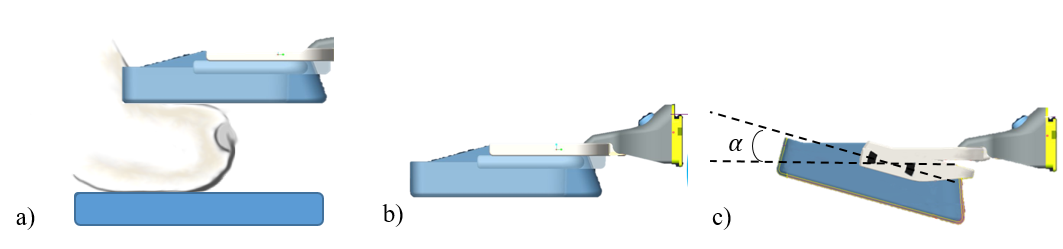
\includegraphics[width=0.9\textwidth,keepaspectratio]{figures/compressionpaddles.png} 
\caption{Breast compression between the paddle (up) and the receiver (down): a) Rigid paddle; b)Flex paddle with flexion angle $\alpha$}\label{fig:compressionpaddles}
\end{figure}




\section{Discussions and Conclusion}\label{section:compression:conclusion}